\documentclass{article}

\usepackage{fancyhdr}
\usepackage{extramarks}
\usepackage{amsmath}
\usepackage{amsthm}
\usepackage{amsfonts}
\usepackage{amssymb}
\usepackage{tikz}
\usepackage[plain]{algorithm}
\usepackage{algpseudocode}

\usetikzlibrary{automata,positioning}

%
% Basic Document Settings
%

\topmargin=-0.45in
\evensidemargin=0in
\oddsidemargin=0in
\textwidth=6.5in
\textheight=9.0in
\headsep=0.25in

\linespread{1.1}

\pagestyle{fancy}
\lhead{\hmwkAuthorName}
\chead{\hmwkClass\ (\hmwkClassInstructor\ | \hmwkClassTime): \hmwkTitle}
\rhead{\firstxmark}
\lfoot{\lastxmark}
\cfoot{\thepage}

\renewcommand\headrulewidth{0.4pt}
\renewcommand\footrulewidth{0.4pt}

\setlength\parindent{0pt}

%
% Create Problem Sections
%

\newcommand{\enterProblemHeader}[1]{
    \nobreak\extramarks{}{Problem \arabic{#1} continued on next page\ldots}\nobreak{}
    \nobreak\extramarks{Problem \arabic{#1} (continued)}{Problem \arabic{#1} continued on next page\ldots}\nobreak{}
}

\newcommand{\exitProblemHeader}[1]{
    \nobreak\extramarks{Problem \arabic{#1} (continued)}{Problem \arabic{#1} continued on next page\ldots}\nobreak{}
    \stepcounter{#1}
    \nobreak\extramarks{Problem \arabic{#1}}{}\nobreak{}
}

\setcounter{secnumdepth}{0}
\newcounter{partCounter}
\newcounter{homeworkProblemCounter}
\setcounter{homeworkProblemCounter}{1}
\nobreak\extramarks{Problem \arabic{homeworkProblemCounter}}{}\nobreak{}

%
% Homework Problem Environment
%
% This environment takes an optional argument. When given, it will adjust the
% problem counter. This is useful for when the problems given for your
% assignment aren't sequential. See the last 3 problems of this template for an
% example.
%
\newenvironment{homeworkProblem}[1][-1]{
    \ifnum#1>0
        \setcounter{homeworkProblemCounter}{#1}
    \fi
    \section{Problem \arabic{homeworkProblemCounter}}
    \setcounter{partCounter}{1}
    \enterProblemHeader{homeworkProblemCounter}
}{
    \exitProblemHeader{homeworkProblemCounter}
}

%
% Homework Details
%   - Title
%   - Due date
%   - Class
%   - Section/Time
%   - Instructor
%   - Author
%

\newcommand{\hmwkTitle}{Homework\ \#5}
\newcommand{\hmwkDueDate}{November 3, 2016}
\newcommand{\hmwkClass}{CS204}
\newcommand{\hmwkClassTime}{Section A}
\newcommand{\hmwkClassInstructor}{Prof. Sungwon Kang}
\newcommand{\hmwkAuthorName}{Ohjun Kwon}

%
% Title Page
%

\title{
    \vspace{2in}
    \textmd{\textbf{\hmwkClass:\ \hmwkTitle}}\\
    \normalsize\vspace{0.1in}\small{Due\ on\ \hmwkDueDate\ at 11:59pm}\\
    \vspace{0.1in}\large{\textit{\hmwkClassInstructor\ | \hmwkClassTime}}
    \vspace{3in}
}

\author{\textbf{20160051 \hmwkAuthorName}}
\date{}

\renewcommand{\part}{\textbf{\large (\alph{partCounter})}\stepcounter{partCounter}\\}

%
% Various Helper Commands
%

% Useful for algorithms
\newcommand{\alg}[1]{\textsc{\bfseries \footnotesize #1}}

% For derivatives
\newcommand{\deriv}[1]{\frac{\mathrm{d}}{\mathrm{d}x} (#1)}

% For partial derivatives
\newcommand{\pderiv}[2]{\frac{\partial}{\partial #1} (#2)}

% Integral dx
\newcommand{\dx}{\mathrm{d}x}

% Alias for the Solution section header
\newcommand{\solution}{\textbf{\large Solution}}

% Probability commands: Expectation, Variance, Covariance, Bias
\newcommand{\E}{\mathrm{E}}
\newcommand{\Var}{\mathrm{Var}}
\newcommand{\Cov}{\mathrm{Cov}}
\newcommand{\Bias}{\mathrm{Bias}}

\newcommand\numberthis{\addtocounter{equation}{1}\tag{\theequation}}

\begin{document}

\maketitle

\pagebreak

\begin{homeworkProblem}
    \part
    \begin{align*}
        H(1)&=1\\
        H(2)&=1\\
        H(3)&=H(2)+H(1)-H(0)\\
        &=1+1-0=2\\
        H(4)&=H(3)+H(2)-H(1)\\
        &=2+1-1=2\\
        H(5)&=H(4)+H(3)-H(2)\\
        &=2+2-1=3\\
        H(6)&=H(5)+H(4)-H(3)\\
        &=3+2-2=3\\
        H(7)&=H(6)+H(5)-H(4)\\
        &=3+3-2=4\\
        H(8)&=H(7)+H(6)-H(5)\\
        &=4+3-3=4\\
        H(9)&=H(8)+H(7)-H(6)\\
        &=4+4-3=5\\
        H(10)&=H(9)+H(8)-H(7)\\
        &=5+4-4=5
    \end{align*}
    \part
    For $n\geq 0$, we can guess that $\displaystyle H(n)=\left\lfloor \frac{n+1}2\right\rfloor$.\\
    $\displaystyle \therefore H(100)=\left\lfloor \frac{100+1}2\right\rfloor=50$
\end{homeworkProblem}

\begin{homeworkProblem}
    \part
    If we draw 3 points on the leftside and $n$ points on the rightside, we can make a complete bipartite graph by connecting all points on the leftside with the points on the rightside.
    Then, we can make $K_{3,n}$ with $K_{3,n-1}$ by adding one point on the right and connect it with all the points on the left side (3 points).
    After doing this job, three more edges are added to the graph.
    So, we can make a recurrence relation based on this.
    $$
    K_{3,n}=K_{3,n-1}+3
    $$

    \part
    We can think of the relation between $K_{n-1,n-1}$ and $K_{n,n}$.
    We can make $K_{n,n}$ from $K_{n-1,n-1}$ by drawing a point on the left side and another point at the right side.
    Then, we should connect them in line. First, we can draw $n$ lines from the left point we have just drawed to the points at the right side.
    Next, we can draw $n-1$ lines from the right point to the points at the right side, because we have already drawn a line in between the new points.
    $\therefore K_{n,n}=K_{n-1,n-1}+2n-1$
\end{homeworkProblem}

\begin{homeworkProblem}
    \textbf{Base case}
    For $n\geq 0$,
    \begin{align*}
        C(0)&=\frac{3^{0+1}-2\cdot 0-3}4\\
        &=0
    \end{align*}
    \qedsymbol
    \\

    \textbf{Inductive case}
    \begin{align*}
        C(n)&=n+3C(n-1)\numberthis \label{eq:1} \\
        &=n+3\cdot \frac{3^n-2(n-1)-3}4\numberthis \label{eq:2} \\
        &=n+3\cdot \frac{3^n-2n-1}4\\
        &=n+\frac{3^{n+1}-6n-3}4\\
        &=\frac{4n}4+\frac{3^{n+1}-6n-3}4\\
        &=\frac{3^{n+1}-2n-3}4
    \end{align*}
    (\ref{eq:1}): recurrence relation\\
    (\ref{eq:2}): inductive hypothesis\\
    \qedsymbol
\end{homeworkProblem}

\begin{homeworkProblem}
    \part
    \begin{align*}
        G(0)&=1\\
        G(1)&=G(0)+2\cdot 1-1\\
        &=1+2-1=2\\
        G(2)&=G(1)+2\cdot 2-1\\
        &=2+4-1=5\\
        G(3)&=G(2)+2\cdot 3-1\\
        &=5+6-1=10\\
        G(4)&=G(3)+2\cdot 4-1\\
        &=10+8-1=17\\
        G(5)&=G(4)+2\cdot 5-1\\
        &=17+10-1=26
    \end{align*}

    \part
    We can make a sequence of differences from the six values.
    Figure~\ref{fig:sod} can be drawn from the sequence.
    \begin{figure}[!ht]
        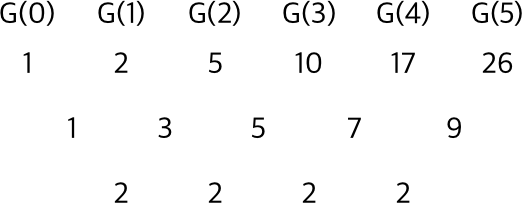
\includegraphics[width=0.5\textwidth]{seq_of_diff}
        \centering
        \caption{sequence of differences}
        \label{fig:sod}
    \end{figure}
    The second sequence of differences is constant.
    This suggests that the sequence may have a formula of the form $G(n)=An^2+Bn+C$.
    If we substitute $n$ with $0$, $1$, $2$, and use $G(0)$, $G(1)$, $G(2)$; then we can make a system of equations like below.
    \begin{align*}
        1&=C\\
        2&=A+B+C\\
        5&=4A+2B+C
    \end{align*}
    We can get $A=1$, $B=0$, $C=1$ from the system.\\
    Therefore, we can assume that $G(n)=n^2+1$.

    \part
    We want to show that the recurrence relation is equal with the hypothesized closed-form formula that we have obtained \textbf{4(b)}.
    Let $G(n)$: the given recurrence relation and $f(n)$: the hypothesized closed-form formula.
    \\

    \textbf{Base formula}
    $G(0)=1=f(0)$
    \qedsymbol

    \textbf{Inductive formula}
    \begin{align*}
        G(n)&=G(n-1)+2n-1\numberthis \label{eq:3} \\
        &=f(n-1)+2n-1\numberthis \label{eq:4} \\
        &=(n-1)^2+1+2n-1\\
        &=n^2-2n+1+2n\\
        &=n^2+1\\
        &=f(n)
    \end{align*}
    (\ref{eq:3}): recurrence relation\\
    (\ref{eq:4}): inductive hypothesis\\
    \qedsymbol
\end{homeworkProblem}

\begin{homeworkProblem}
    Applying the rule recursively, we can get a set $\mathbb{Z}$.
    \begin{align*}
        \mathbb{Z}=\{&(1,5),(1,7),(1,9),\\
        &(2,4),(2,6),(2,8),(2,10),\\
        &(3,5),(3,7),(3,9),\\
        &(4,6),(4,8),(4,10),\\
        &(5,7),(5,9),\\
        &(6,8),(6,10),\\
        &(7,9),\\
        &(8,10)\}
    \end{align*}
    \begin{figure}[!ht]
        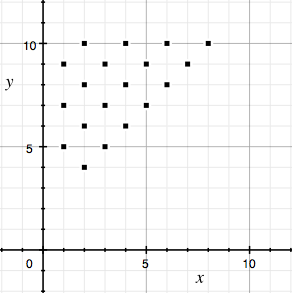
\includegraphics[width=0.3\textwidth]{5_graph}
        \centering
        \caption{a plot of the set $\mathbb{Z}$}
    \end{figure}
\end{homeworkProblem}

\begin{homeworkProblem}
    \part
    $\varnothing$, $\{\varnothing\}$, $\{\{\varnothing\}\}$

    \part
    If the set $S$ has an element $x$, then $S$ should contain a set which has the element $x$ as an element, i.e. $\{x\}\in S$,
    since $\{x\}$ is a subset of $S$. However, this rule is applied to the all elements that are added to the $S$ recursively.
    For example, if $x$ is in $S$, $\{x\},\{\{x\}\},\dots$ should also be the elements of the set $S$.
    Therefore, the set $S$ has infinitly many elements.
\end{homeworkProblem}
\pagebreak
\begin{homeworkProblem}
\end{homeworkProblem}
\pagebreak
\begin{homeworkProblem}
    \textbf{Base case}
    For $n=1$ (odds' base case),
    \begin{align*}
        H(2\cdot 1)&=H(2)=1\\
        H(2\cdot 1 - 1)&=H(1)=1\\
        n &= 1
    \end{align*}
    $\therefore H(2n)=H(2n-1)=n$ for $n=1$ \qedsymbol
    \\

    For $n=2$ (evens' base case),
    \begin{align*}
        H(2\cdot 2 - 1)&=H(3)=H(2)+H(1)-H(0)\\
        &=1+1-0=2\\
        H(2\cdot 2)&=H(4)=H(3)+H(2)-H(1)\\
        &=2+1-1=4\\
        n &= 2
    \end{align*}
    $\therefore H(2n)=H(2n-1)=n$ for $n=2$ \qedsymbol \\

    \textbf{Inductive case}\\
    \textbf{i) n is even}
    Let $n=2k$,
    \begin{align*}
        H(n)&=H(2k)\\
        &=H(2k-1)+H(2k-2)-H(2k-3)\numberthis \label{eq:q1} \\
        &=H(2k-1)+H(2(k-1))-H(2(k-1)-1)\\
        &=k+(k-1)-(k-1)\numberthis \label{eq:q2} \\
        &=k
    \end{align*}

    \textbf{ii) n is odd}
    Let $n=2k-1$,
    \begin{align*}
        H(n)&=H(2k-1)\\
        &=H(2k-2)+H(2k-3)-H(2k-4)\numberthis \label{eq:q3} \\
        &=H(2(k-1))+H(2(k-1)-1)-H(2(k-2))\numberthis \label{eq:q4} \\
        &=(k-1)+(k-1)-(k-2)\\
        &=k
    \end{align*}

    (\ref{eq:q1}), (\ref{eq:q3}): recurrence relation\\
    (\ref{eq:q2}), (\ref{eq:q4}): inductive hypothesis
\end{homeworkProblem}
\pagebreak
\begin{homeworkProblem}
\end{homeworkProblem}
\pagebreak
\begin{homeworkProblem}
    \textbf{Base case}
    For a element from Q-sequence $<x,4-x>$, $x+(4-x)=4$. Therefore, the condition holds.

    \textbf{Inductive case}
    Suppose $<x_1,x_2,\dots ,x_j>$ and $<y_1,y_2,\dots ,y_k>$ is a Q-sequence.\\
    Then, $x_1+x_2+\dots +x_j=4$ and $y_1+y_2+\dots +y_k=4$ by the induction hypothesis.\\
    For $<x_1-1,x_2,\dots ,x_j,y_1,y_2,\dots ,y_{k-1},y_k-3>$, the sum of the number is
    \begin{align*}
        &x_1-1+x_2+\dots +x_j+y_1+\dots +y_{k-1}+y_k-3\\
        &=x_1+x_2+\dots +x_j+y_1+y_2+\dots +y_{k-1}+y_k-4\\
        &=4+4-4=4
    \end{align*}
    $\therefore$ the proposition holds. \qedsymbol
\end{homeworkProblem}
\end{document}
